\section{Специализированные инструменты}

\subsection{funccount}
Подсчитывает события, в частности вызовы функций. \\

\noindent Примеры использования:\\
\noindent Вызывается ли функция tcp\_drop()? \\
\ci{\# funccount tcp\_drop}
\noindent Какая функция из подсистемы VFS в ядре вызывается чаще всего? \\
\ci{\# funccount 'vfs\_*'}
\noindent Сколько раз в секунду вызывается функция pthread\_mutex\_lock() в пространстве пользователя? \\
\ci{\# funccount -i 1 c:pthread\_mutex\_lock}
\noindent Какая из строковых функций в libc вызывается чаще всего в системе в целом? \\
\ci{\# funccount 'c:str*'}
\noindent Какой системный вызов вызывается чаще всего? \\
\ci{\# funccount 't:syscalls:sys\_enter\_*'}
\noindent Подсчет вызовов функций виртуальной файловой системы в ядре:\\
\ci{\# funccount 'vfs\_*'}
\noindent Подсчет вызовов функций TCP в ядре:\\
\ci{\# funccount 'tcp\_*'}
\noindent Определение частоты вызовов в секунду функций TCP:\\
\ci{\# funccount -i 1 'tcp\_send*'}
\noindent Определение частоты операций блочного ввода/вывода в секунду:\\
\ci{\# funccount -i 1 't:block:*'}
\noindent Определение частоты запуска новых процессов в секунду:\\
\ci{\# funccount -i 1 t:sched:sched\_process\_fork}
\noindent Определение частоты вызовов в секунду функции getaddrinfo() (разрешение имен)
из библиотеки libc:\\
\ci{\# funccount -i 1 c:getaddrinfo}
\noindent Подсчет вызовов всех функций «os.*” в библиотеке libgo:\\
\ci{\# funccount 'go:os.*'}

\subsection{stackcount}

Подсчитывает трассировки стека, которые привели к событию. \\

\noindent Пример использования stackcount для определения путей выполнения кода,
ведущих к вызову ktime\_get(): \\
\ci{\# stackcount ktime\_get}

\noindent Параметр -P позволяет добавить имена и идентификаторы PID процессов:\\
\ci{\# stackcount -P ktime\_get}

\noindent Создание флейм-графиков: \\
\ci{\# stackcount -f -P -D 10 ktime\_get > out.stackcount01.txt}
\ci{\$ git clone http://github.com/brendangregg/FlameGraph}
\ci{\$ cd FlameGraph}
\ci{\$ ./flamegraph.pl --hash --bgcolors=grey $\backslash$} 
\ci{\indent < ../out.stackcount01.txt > out.stackcount01.svg }
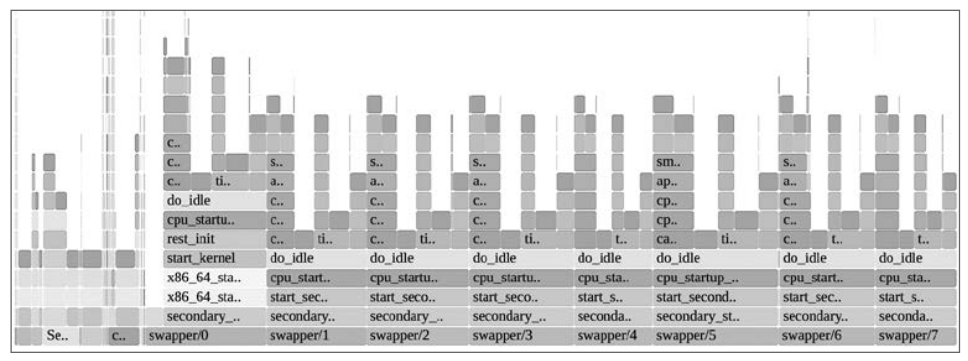
\includegraphics[width=1.0\linewidth]{flame_ktime_get.png}

\noindent\textbf{Однострочные сценарии stackcount} \\
Подсчет трассировок стека, приводящих к операции блочного ввода/вывода: \\
\ci{stackcount t:block:block\_rq\_insert}
Подсчет трассировок стека, приводящих к отправке IP-пакетов: \\
\ci{stackcount ip\_output}
Подсчет трассировок стека, приводящих к отправке IP-пакетов, с разделением по PID: \\
\ci{stackcount -P ip\_output}
Подсчет трассировок стека, приводящих к блокировке потока и переходу в режим ожидания: \\
\ci{stackcount t:sched:sched\_switch}
Подсчет трассировок стека, приводящих к системному вызову read(): \\
\ci{stackcount t:syscalls:sys\_enter\_read}


\subsection{trace}

Многофункциональный инструмент BCC для трассировки отдельных
событий из разных источников: kprobes, uprobes, tracepoints и USDT. \\

\noindent Перехват событий открытия файлов: \\
\ci{\# trace 'do\_sys\_open "\%s", arg2'}
\noindent Трассировка вызовов функции do\_sys\_open() с выводом имен открываемых файлов: \\
\ci{\# trace 'do\_sys\_open "\%s", arg2'}
\noindent Трассировка возврата из функции ядра do\_sys\_open() с выводом возвращаемого значения: \\
\ci{\# trace 'r::do\_sys\_open "ret: \%d", retval'}
\noindent Трассировка функции do\_nanosleep() с выводом аргумента режима и трассировкой стека в пространстве пользователя: \\
\ci{\# trace -U 'do\_nanosleep "mode: \%d", arg2'}
\noindent Трассировка запросов в библиотеку pam на аутентификацию: \\
\ci{\# trace 'pam:pam\_start "\%s: \%s", arg1, arg2'}

\noindent \textbf{trace и структуры:} \\
\cn{\# trace -I 'net/sock.h' $\backslash$}
\ci{udpv6\_sendmsg(struct sock *sk) (sk->sk\_dport == 13568)'}

\noindent Использование trace для отладки утечек дескрипторов файлов: \\
\ci{\# trace -tKU 'r::sock\_alloc "open \%llx", retval' $\backslash$}
\ci{\indent '\_\_sock\_release "close \%llx", arg1' }

\subsection{argdist}
Многофункциональный инструмент, который суммирует аргументы. \\

\noindent Гистограмма распределения размеров окна: \\
\ci{\# argdist -H 'r::\_\_tcp\_select\_window():int:\$retval'}

\noindent Вывести гистограмму результатов (размеров), возвращаемых функцией ядра vfs\_read(): \\
\ci{\# argdist.py -H 'r::vfs\_read()'}
\noindent Вывести гистограмму результатов (размеров), возвращаемых функцией read() из библиотеки libc в пространстве пользователя для PID 1005: \\
\ci{\# argdist -p 1005 -H 'r:c:read()'}
\noindent Подсчитать число обращений к системным вызовам по их идентификаторам с ис- пользованием точки трассировки raw\_syscalls:sys\_enter: \\
\ci{\# argdist.py -C 't:raw\_syscalls:sys\_enter():int:args->id'}
\noindent Подсчитать значения аргумента size для tcp\_sendmsg(): \\
\ci{\# argdist -C 'p::tcp\_sendmsg(struct sock *sk, $\backslash$}
\ci{\indent \indent struct msghdr *msg, size\_t size):u32:size'}
\noindent Вывести гистограмму распределения значений аргумента size в вызовах tcp\_ sendmsg(): \\
\ci{\# argdist -H 'p::tcp\_sendmsg(struct sock *sk, $\backslash$ }
\ci{\indent \indent  struct msghdr *msg, size\_t size):u32:size'}
\noindent Подсчитать количество вызовов функции write() из библиотеки libc для PID 181 по дескрипторам файлов: \\
\ci{\# argdist -p 181 -C 'p:c:write(int fd):int:fd'}
